\section{Methods}
\label{sec:methods}

Figure \ref{rider_system} provides an overview of the training and evaluation procedure for the classification models in the current study. Subsequent Sections will offer detailed explanations for each step.

\begin{figure}[htbp]
\centering
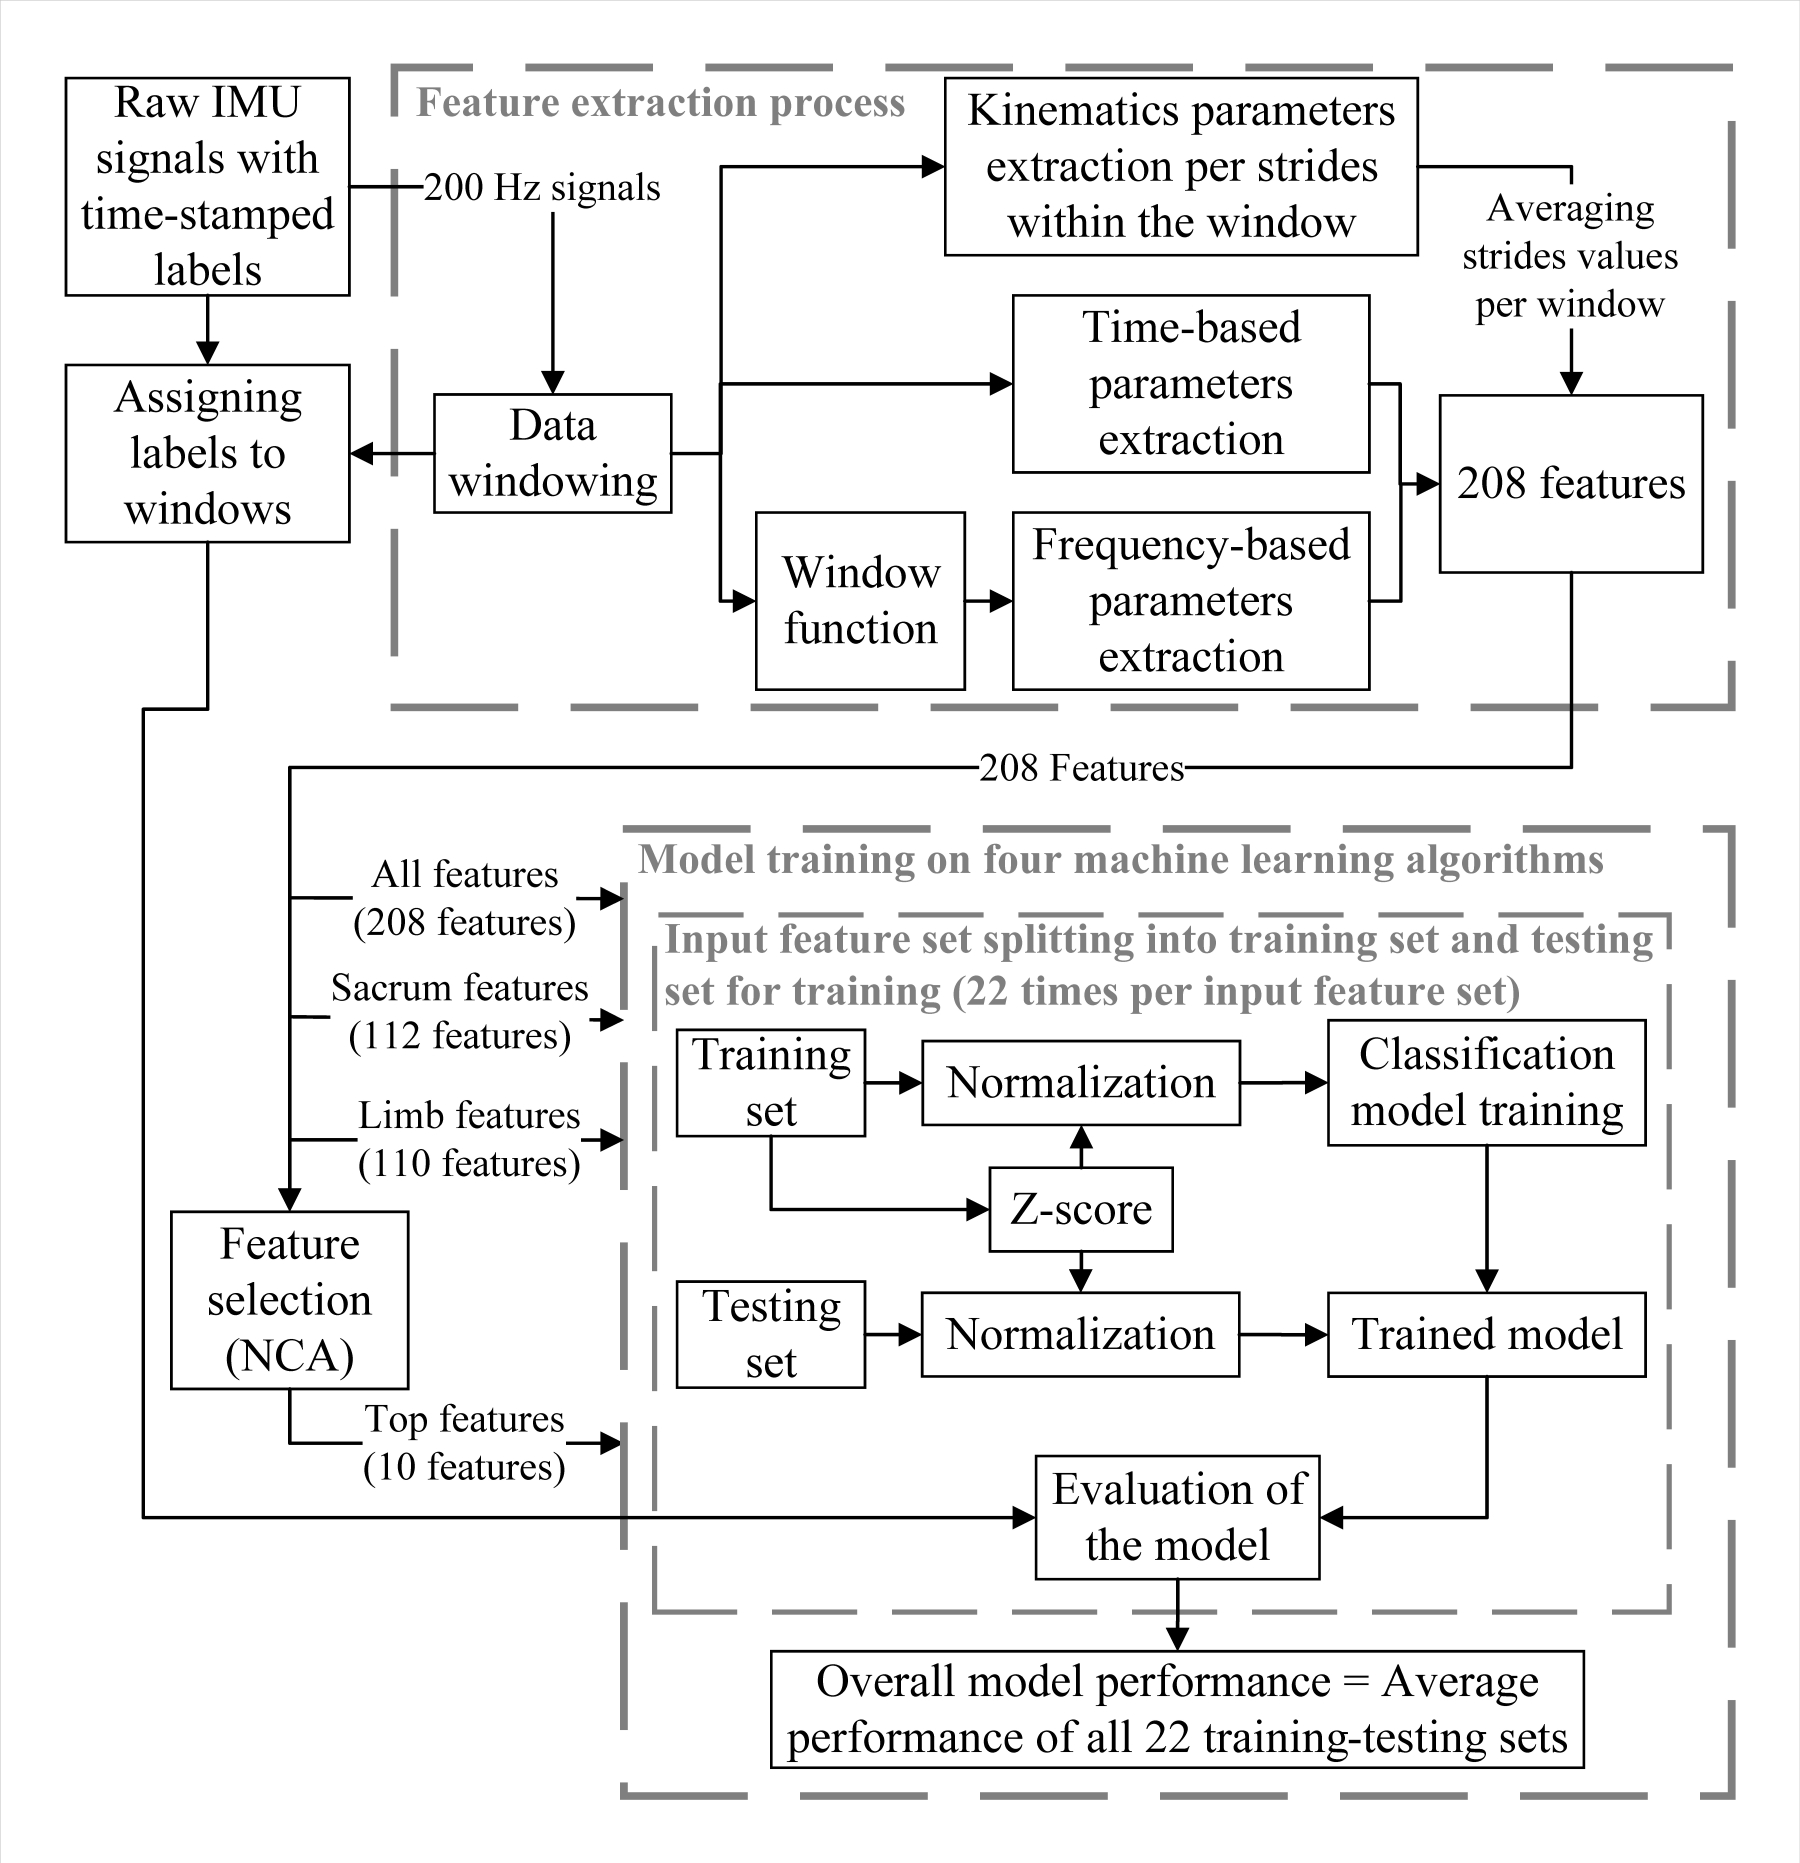
\includegraphics[width=\linewidth]{chapters/rider/figures/system.jpg}
\caption{A summary of model training and evaluating procedure.}
\label{rider_system}
\end{figure}

\subsection{Data preparation}
%\subsection{Data}
\label{subsec:data}
The data used in this study were collected from twenty-two Warmblood eventing horses walking and trotting ridden and not ridden. The Animal Ethics Committee of Utrecht University concluded that ethical approval was not needed for the data collection since it did not qualify as an animal experiment. Horses were equipped with two ProMove-mini  (Inertia Technology B.V., Enschede, The Netherlands) \gls{imu} on the sacrum and right front limb (cannon bone). Each \gls{imu} contained a tri-axial accelerometer and a tri-axial gyroscope. The \gls{imu}s were equipped on the sacrum and right front limb (cannon bone). For conciseness, we address the right front limb as “limb” in this chapter. \gls{imu}s were set to collect data at a sampling rate of 200 Hz, a low-acceleration range of ±16 g, a high-acceleration range of ±200 g, and an angular velocity of 2000 deg/s. 

Figure \ref{fig:two IMU on horse} demonstrates the \gls{imu} locations and orientations on the horse's body. The three axes of rotation for the sacrum \gls{imu} were x, y, and z, which were defined in the order of longitudinal axis, mediolateral axis, and vertical axis. For the limb, the x-axis was aligned to the cannon bone (vertical axis), the y-axis was assigned as the retraction/protraction angle axis of rotation (longitudinal axis), and the z-axis was used as the abduction/adduction angle axis of rotation (mediolateral axis).

\begin{figure}[htbp]
\centering
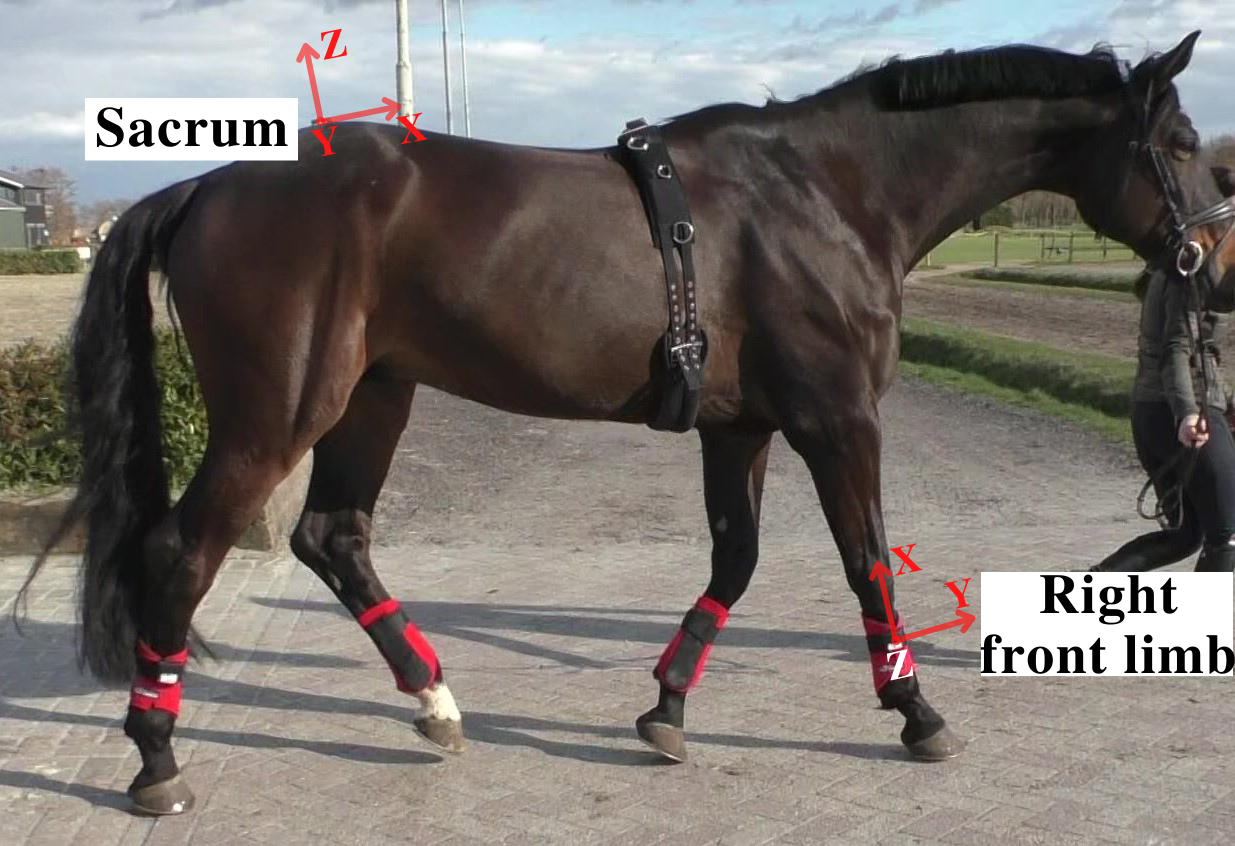
\includegraphics[width=.75\linewidth]{chapters/fatigue/figures/Picture7.png}
\caption{\gls{imu}s locations and orientations on horse body.}
\label{fig:two IMU on horse}
\end{figure}


%\subsection{Data labeling}
Through the presence on the field and meticulous observation of measurements, we recorded the timestamps marking the start and end of riding sessions. Following the extraction of signals from both the sacrum and limb \gls{imu}s, we partitioned them into distinct time segments based on the recorded timestamps. Each of these segments was then labeled to indicate whether the horse was being ridden or not-ridden.

%\subsection{Dataset preparation}

We prepared the extracted signals in two versions, raw and filtered-rotated. The raw signals were received from \gls{imu}s without any modifications. For preparing the filtered-rotated version, the raw signals were first low-pass filtered using a fourth-order Butterworth filter and 30 Hz cut-off frequency. Then the local orientation of the \gls{imu} was rotated to a global orientation, where the z-axis was aligned with the gravity vector. 
 
 Both versions of signals were time-synchronized. The raw signals were used for almost all the calculations in this chapter, except for the calculation of the parameters related to the sacrum \gls{imu} vertical displacement. The acceleration signals of sacrum \gls{imu} were filtered and rotated for the purpose of calculating sacrum vertical displacement and its related parameters, which are discussed in Section \ref{sec:Extraction of kinematic parameters}. 
	
The size of the model input was considered as a 2.56-second window of signals, equivalent to 512 timesteps. Using a sliding step of 128 timesteps, 512 timesteps windows were extracted from raw and filtered-rotated signals. Thus, subsequent windows were overlapped by 75 percent. The overlapping helps to enumerate the data size and adapt the model to different windows of signals. Since the entire dataset had been partitioned and labeled manually in advance, the generated windows were also assigned "ridden" and "not-ridden" labels.
	
%\subsection{Extraction of time and frequency-domain parameters}
\subsection{Feature extraction}
\label{sec:Extraction of kinematic parameters}

Based on the features selected in similar machine learning-based studies \cite{ahmed_2020_enhanced,barwick_2018_predicting,rehman_2019_selecting,kamminga_2018_robust}, sixteen time- and frequency-domain parameters were extracted from the windows of each signal. These parameters are presented in Table \ref{tab:features_rider}. All the frequency-domain parameters were based on the derivatives of \gls{fft}. Therefore, before the computation of frequency-domain parameters, the von Hann function was implemented on the windows to reduce spectral leakage and enhance the outcome.

\input{../tables/features_rider.tex}

%\subsection{Extraction of kinematic parameters} 

Sixteen kinematic parameters per stride were selected for this study and are presented in Table \ref{tab:parameters_rider}. These parameters were frequently discussed in equine gait analysis literature, and their analysis is essential for equine health and performance evaluation. We determined stride, stance, and swing duration according to Table \ref{tab:stride_related_parameters}. The hoof-on and hoof-off moments were estimated using the stride event detection algorithm introduced in Chapter \ref{chapter:Step},  in which the inputs are the acceleration and angular velocity signals from the
limb \gls{imu}. Speed was estimated using the estimation model introduced in Chapter \ref{chapter:Speed}, which receives acceleration and angular velocity signals of the sacrum or limb \gls{imu}s as input. 

\begin{table}[!htbp] 
\centering
\caption{Time- and frequency-domain parameters}% Add 'table' caption
\resizebox{\linewidth}{!}{%
\begin{tabular}{m{5cm}m{3cm}ccc}
\toprule
&&\multicolumn{3}{c}{\textbf{Number of parameters per dataset}}\\
\cline{3-5}
\multicolumn{1}{l}{\textbf{Parameter}} & \multicolumn{1}{l}{\textbf{Based on ...}} &  \multicolumn{1}{l}{\textbf{Sacrum \gls{imu}}} & \multicolumn{1}{l}{\textbf{Limb \gls{imu}}} & \multicolumn{1}{l}{\textbf{Both \gls{imu}s}}\\
\midrule 
    
\multicolumn{1}{l}{Stride, stance, and swing duration}  & \multicolumn{1}{l}{Sacrum or limb \gls{imu}s} & 3 & 3 & 3\\
\multicolumn{1}{l}{Speed}  & \multicolumn{1}{l}{Sacrum or limb \gls{imu}s}  & 1 & 1 & 1\\
\multicolumn{1}{l}{AROM around the IMU three axes}  & \multicolumn{1}{l}{Sacrum and limb \gls{imu}s}  & 3 & 3 & 6\\
\multicolumn{1}{l}{LROM along the x- and z-axes of \gls{imu}s}  & \multicolumn{1}{l}{Sacrum and limb \gls{imu}}  & 2 & 2 & 4\\
\multicolumn{1}{l}{MaxDiff and MinDiff}  & \multicolumn{1}{l}{Sacrum \gls{imu}} & 2&-&2\\
&\multicolumn{1}{c}{\textbf{Total}}  & \textbf{11}&\textbf{9}&\textbf{16}\\
        \bottomrule         
        
    \label{tab:parameters_rider}
  \end{tabular}
  }

\end{table}

For the angular range of motion, first, the angular velocity signals from \gls{imu}s per stride were time-integrated to create an angle signal. Then, the difference between maximum and minimum values within each stride was assigned as the angular range of motion of the stride. The limb orientation around its three axes (protraction/retraction, adduction/abduction, and internal/external rotation) was considered as if the limb was the cannon bone, the carpal joint as the reference point, and axes as depicted and described in section \ref{subsec:data}. Also, the angular ranges of motion around the three axes of pelvis (roll, yaw, and pitch) were determined by considering the rotation reference point as the center of the \gls{imu} and its axes, as depicted in Figure \ref{fig:two IMU on horse}. 

To calculate the displacement parameters, we applied a cyclical integration process on acceleration signals, which is described in \cite{pfau_2005_a}. After generating the \gls{imu}s displacement signals during all strides, the mediolateral and vertical linear range of motion of the sacrum (y- and z-axes) and limb (x- and z-axes) were determined by calculating the difference between maximum and minimum values of displacements signals within each stride. Finally, the differences between the two maxima (MaxDiff) and the two minima (MinDiff) of sacrum vertical displacement within a stride were calculated. 

All the mentioned kinematic parameters were defined based on full strides, i.e. flexible-size windows. On the other hand, the extraction of time- and frequency-domain parameters was based on fixed-size windows. The window sizes (512 timesteps) were large enough to contain at least one full walking or trotting stride and at most two full walking or three full trotting strides. Therefore, we time-synchronized the parameters extracting the kinematic parameters from the full strides within each window and assigning their average value as the parameter value for the window in cases where there were multiple strides.

%\subsection{Dataset preparation}
We merged the time- and frequency-domain parameters with kinematic parameters to prepare the input features for the classification model. Sixteen time- and frequency-domain parameters were extracted from the windows of each signal, and six signals per \gls{imu} added up to 192 parameters. By adding the 16 gait kinematic parameters, the number of input features reached 208. In addition to the model based on both \gls{imu}s parameters, one model based on sacrum \gls{imu} parameters and one model based on limb \gls{imu} parameters were also trained. These two models consisted of 16 time- and frequency-domain parameters from each of their six signals (96 parameters) plus the kinematic parameters that were calculated based on the signals. According to the right column of Table \ref{tab:parameters_rider}, 11 and 9 kinematic parameters were extracted from the sacrum and limb \gls{imu}s, respectively. In total, 107 and 105 input features were gathered for training the sacrum \gls{imu} and limb \gls{imu} models.

%\subsection{Feature selection}
The importance of kinematic and time- and frequency-domain parameters was measured by implementing a \gls{nca} on the data of each horse separately. By considering the weights of the features from the \gls{nca} output as the “importance” meter, the ten parameters with the highest weights were selected as the ten most important parameters in distinguishing ridden and not-ridden data per subject. Then, ten parameters that presented the most in all subjects were selected as the most important parameters overall.

\subsection{Model training, testing, and optimization}
Three classification models based on Sacrum+Limb \gls{imu}s, sacrum \gls{imu}, and limb \gls{imu} features were trained on each training dataset and tested using the dedicated testing dataset and its derivatives (walking and trotting testing datasets). \gls{svm}, \gls{lda}, decision tree, and random forest were appointed as the machine learning algorithms.

Equal to the number of subjects, twenty-two training-testing datasets were created from the parameters; each dataset consisted of twenty-one subjects as a training dataset and one as a testing dataset. For each training-testing dataset, the training dataset was normalized using Z-score (equation \ref{eq:zscore}). Then, by using the generated Z-score, the testing dataset was normalized afterward. Leaving one subject out of training datasets and normalizing the training-testing dataset by only using the training dataset prevents the model from overfitting. It should be noted that the models were trained based on a combination of walking and trotting, identified as Walk+Trot. For comparison of model performance based on gait, one only walking and one only trotting testing dataset was derived from each testing dataset.

To study the impact of important parameters on the performance of classification models and to assess how resource constraints for the purpose of optimization affect model performance, one model for each of the four selected machine learning algorithms was also trained by using only the top ten selected parameters (by \gls{nca}) as model input features using Sacrum+Limb data during Walk+Trot. 

The testing process yielded confusion matrices, which were used to calculate the sensitivity, specificity, and accuracy of the three models. The confusion matrix elements are the number of true positives (correct ridden predictions), true negatives (correct not-ridden predictions), false positives (when the model incorrectly predicts ridden as not-ridden), and false negatives (when the model incorrectly predicts not-ridden as ridden). MATLAB R2021b (MathWorks Inc., Natick, MA, USA) was used for all the calculations and modeling.